\section{Formulating duals}

In this chapter, we will discuss the notion of duality, under the context of linear programming problem. Duality can be understood as a property that makes available a collection of tools and features that can be exploited to both further understand characteristics of the optimal solution and to devise specialised methods for solving large-scale linear programming problems.


\subsection{Motivation}

Let us define the notation we will be using throughout the next chapters. As before, let $c \in \reals^n$, $b \in \reals^m$, $A \in \reals^{m \times n}$, and $P$ be the standard form linear programming problem
%
\begin{align*}
	(P) : \mini \ & c^\top x \\
	\st 	  & Ax = b \\
		  & x \geq 0,   
\end{align*}
%
which we will refer to as the \emph{primal} problem.  In mathematical programming, we say that a constraint has been \emph{relaxed} if it has been removed from the set of constraints. With that in mind, let us consider a \emph{relaxed} version of $P$, where $Ax = b$ is replaced with a \emph{violation penalty} term $p^\top (b - Ax)$. This lead to the following problem:
%
\begin{equation*}
	g(p) = \mini_{x \geq 0} \braces{c^\top x + p^\top (b - Ax)},
\end{equation*}
%
which has the benefit of not having equality constraints explicitly represented, but only implicit by means of a penalty element that can be used to penalise infeasibility of the constraints in the attempt to steer the solution of this relaxed problems towards the solution to $P$. Recalling that our main objective is to solve $P$, we are interested in the values (or prices, as they are often called) for $p \in \reals^m$ that make $P$ and $g(p)$ equivalent.

Let $\overline{x}$ be the optimal solution to $P$. Notice that, for any $p \in \reals^m$, we have that
%
\begin{equation*}
	g(p) = \mini_{x \geq 0} \braces{c^\top x + p^\top (b - Ax)} \leq c^\top \overline{x} +  p^\top (b - A\overline{x}) = c^\top \overline{x},   
\end{equation*}
%
i.e., $g(p)$ is a \emph{lower bound} on the optimal value $c^\top \overline{x}$. The lefthand-side inequality holds because, although $\overline{x}$ is optimal for $P$, it might not be optimal for $g(p)$ for an arbitrary vector $p$. The second inequality is a consequence of $\overline{x} \in P$, i.e., the feasibility of $\overline{x}$ implies that $A\overline{x} = b$.

We can use an optimisation-based approach to try to find an optimal lower bound, i.e., the tightest possible lower bound for $P$. this can be achieved by solving the \emph{dual problem} $D$ formulated as 
%
\begin{equation*}
	(D) : \maxi_p g(p).
\end{equation*}
%
Notice that $D$ is an unconstrained problem, to which a solution proves the \emph{tightest} lower bound on $P$ (say, at $\overline{p}$). Also, notice how the function $g(p) : \reals^m \mapsto \reals$ has embedded on its evaluation the solution of a linear programming problem with $x \in \reals^n$ as decision variables for a fixed $p$, which is the argument given to the function $g$. This is a new concept at this point that often is a source of confusion. 

We will proceed in this chapter developing the analytical framework that allows use to pose the key result in duality theory, which is that stating that 
%
\begin{equation*}
	g(\overline{p}) = c^\top \overline{x}.	
\end{equation*}
%
That is, we will next develop the results that guarantee the equivalence between primal and dual representations. This will be useful for interpreting properties associated with the optimal primal solution $\overline{x}$ from the associated optimal prices $\overline{p}$. Furthermore, we will see in later chapters that linear programming duality can be used as a framework for replacing constraints with equivalent representations, which is a useful procedure in many settings, including for developing alternative solution strategies also based in linear programming. 


\subsection{General form of duals}

Now, let us focus on developing a formulation for dual problems that is based on linear programming as well. Using the definition of $D$, we notice that
%
\begin{align*}
	g(p) = \ & \mini_{x \geq 0}  \braces{c^\top x + p^\top (b - Ax)}	\\
	= \ & p^\top b + \mini_{x \geq 0}  \braces{c^\top x - p^\top Ax}    \\
    = \ & p^\top b + \mini_{x \geq 0}  \braces{(c^\top - p^\top A)x}.  
\end{align*} 
%
As $x \ge 0$, the rightmost problem can only be bounded if $(c^\top - p^\top A) \ge 0$. This gives us a linear constraint that can be used to enforce the existence of a solution for 
%
\begin{equation*}
	\mini_{x \geq 0}  \braces{(c^\top - p^\top A)x}.
\end{equation*}
%
With that in mind, we can equivalently reformulate $D$ as
%
\begin{align*}
	(D) : \maxi \ & p^\top b \\
	\st 	  & p^\top A \leq c^\top.
\end{align*}	
%
Notice that $D$ is a linear programming problem with $m$ variables (one per constraint of the primal problem $P$) and $n$ constraints (one per variable of $P$). As you might suspect, if you were to repeat the analysis, looking at $D$ as the ``primal'', you would end with a dual that is exactly $P$. For this to become more apparent, let us fist define more generally the rules that dictate what kind of dual formulations are obtained for different types of primal problems in terms of its original variables and constraints. 

In the more general case, let $P$ be defined as
%
\begin{align*}
	(P) : \mini \ & c^\top x \\
	\st 	  & Ax \geq b.  
\end{align*}
%
Notice that the problem $P$ can be equivalently reformulated as
%
\begin{align*}
	(P) : \mini \ & c^\top x \\
	\st & Ax - s = b \\
	& s \geq 0.
\end{align*}
%
Let us focus on the constraints in the reformulated version of $P$, which can be written as
%
\begin{equation*}
	[A \mid -I] \begin{bmatrix} x \\ s \end{bmatrix} = b. 
\end{equation*}
%
We will apply the same procedure as before, being our constraint matrix $[A \mid -I]$ in place of $A$ and $[x \mid s]^\top$ our vector of variables, in place of $x$. Using analogous arguments, we now require $c^\top - p^\top A = 0$ so $g(p)$ is finite. Notice that this is a slight deviation from before, but is this case we have that $x \in \reals^n$, so $c^\top - p^\top A = 0$ is the only condition that allow the inner problem in $g(p)$ to have a finite solution. Then, we obtain the following dual linear programming formulation
%
\begin{align*}
	&p^\top [A \mid -I] \leq [c^\top \mid 0^\top]  \\
	&c^\top - p^\top A = 0, 
\end{align*}
%
or simply
%
\begin{align*}
	(D) : \maxi \ & p^\top b  \hspace{1.5cm}\\ 
	\st & p^\top A = c^\top \\
	& p \geq 0.
\end{align*}

Notice how the change in the type of constraints in the primal problem $P$ lead to additional nonnegative constraints in the dual variables $p$. Similarly, the absence of explicit nonnegativity constraints in the primal variables $x$ lead to equality constraints in the dual problem $D$, as opposed to inequalities. 

Table \ref{p1c5:tab:primal-dual_conversion} provides a summary which allows one to identify the resulting formulation of the dual problem based on the primal formulation, in particular regarding its type (minimisation or maximisation), constraint types and variable domains.

\begin{table}[h]
	\begin{tabular}{|c|c|} \hline
		{\bf Primal (dual)} & {\bf Dual (primal)} \\ \hline
		 minimise & maximise \\
		Independent terms  & Obj. function coef.  \\
		Obj. function coef.  & Independent terms  \\
		$i$-th row of constraint coef. & $i$-th column of constraint coef. \\
		$i$-th column of constraint coef. & $i$-th row of constraint coef. \\ \hline
		{\bf Constraints} & {\bf Variables} \\ \hline
		$\geq$ & $\geq 0$ \\
		$\leq$ & $\leq 0$ \\
		$=$ & $\in \reals$ \\ \hline
		{\bf Variables} & {\bf Constraints} \\ \hline
		$\geq 0$ & $\leq$ \\
		$\leq 0$ & $\geq$ \\
		$\in \reals$ & $=$ \\ \hline
	\end{tabular}
	\caption{Primal-dual conversion table} \label{p1c5:tab:primal-dual_conversion}
\end{table}

For converting a minimisation primal problem into a (maximisation) dual, one must read the table from left to right. That is, the independent terms ($b$) become the objective function coefficients, greater or equal constraints become nonnegative variables, and so forth. However, if the primal problem is a maximisation problem, then the table must be read from right to left. For example, in this case, less-or-equal-than constraints would be come nonnegative variables instead, and so forth. It takes a little practice to familiarise yourself with this table, but it turns to be a really useful resource to obtain dual formulations from primal problems.

One remark to be made at this point is that, as is hopefully clearer now, the conversion of primal problems into duals is symmetric, meaning that reapplying the rules in Table \ref{p1c5:tab:primal-dual_conversion} would take you from the obtained dual back to the original primal. This is a property of linear programming problems and is called being \emph{self dual}. Another remark is that equivalent reformulations made in the primal lead to equivalent duals. Specifically, transformations that replace variables $x \in \reals$ with $x^+ - x^-$, with $x^+, x^- \geq 0$, introduce of nonnegative slack variables, or remove redundant constraints lead to equivalent duals. 

For example, recall that the dual formulation for the primal problem 
%
\begin{align*}
	(P) : \mini \ & c^\top x \\
	\st &Ax \geq b \\
	&x \in \reals^n
\end{align*}
%
is given by
%
\begin{align*}
	(D) : \maxi \ & p^\top b \\
	\st &p \geq 0 \\
	&p^\top A = c^\top. 
\end{align*}
%
Now suppose we equivalently reformulate the primal problem to become
\begin{align*}
	(P') : \mini \ & c^\top x + 0^\top s \\
	\st &A x - s = b \\
	&x \in \reals^n, s \geq 0.
\end{align*}
%
Then, using Table \ref{p1c5:tab:primal-dual_conversion}, we would obtain the following dual formulation, which is equivalent to $D$
\begin{align*}
	(D') : \maxi \ & p^\top b \\
	\st &p \in \reals^m \\
	&p^\top A = c^\top \\
	-&p \leq 0.
\end{align*}
%
Analogously, suppose we were to equivalently reformulate $P$ as 
%
\begin{align*}
	(P'') : \mini \ & c^\top x^+ - c^\top x^- \\
	\st &Ax^+ - Ax^- \geq b \\
	&x^+ \geq 0, x^- \geq 0.
\end{align*}
%
Then, the dual formulation for $P''$ would be 
%
\begin{align*}
	(D'') : \maxi \ & p^\top b \\
	\st &p \geq 0 \\
	&p^\top A \leq c \\
	-&p^\top A \leq -c^\top,
\end{align*}
%
which is also equivalent to $D$.


\section{Duality theory}

We now will develop the technical results associated with duality that will be the kingpin for its use as a framework for devising solution methods and interpreting optimal solution properties. 

\subsection{Weak duality}

Weak duality is the property associated with the bounding nature of dual feasible solutions. This is stated in Theorem \ref{p1c5:thm:weak_duality}.

\begin{theorem}[Weak duality] \label{p1c5:thm:weak_duality}
		Let $x$ be a feasible solution to $(P) : \mini\braces{c^\top x : Ax = b, x \geq 0}$ and $p$ be a feasible solution to $(D) : \maxi\braces{p^\top b : p^\top A \leq c^\top}$, the dual problem of $P$. Then $c^\top x \geq p^\top b$.
\end{theorem}

\begin{proof}
	Let $I = \braces{i}_{i=1}^m$ and $J = \braces{j}_{j=1}^n$. For any $x$ and $p$, define
%
	  	\begin{equation*}
			u_i = p_i (a_i^\top x - b_i) \text{ and }
			v_j = (c_j - p^\top A_j)x_j.	
		\end{equation*}
%
	Notice that $u_i \geq 0$ for $i \in I$ and $v_j \geq 0$ for $j \in J$, since each pair of terms will have the same sign. Thus, we have that
%
	\begin{equation*}
		0 \leq \sum_{i \in I} u_i + \sum_{j \in J} v_j = [p^\top Ax - p^\top b] + [c^\top x - p^\top Ax] = c^\top x - p^\top b. \qedhere
	\end{equation*}
%
\end{proof}

Let us also pose some results that are direct consequences of Theorem \ref{p1c5:thm:weak_duality}, which are summarised in Corollary \ref{p1c5:cor:weak_duality}.

\begin{corollary}[Consequences of weak duality]\label{p1c5:cor:weak_duality}
	The following are immediate consequences of Theorem \ref{p1c5:thm:weak_duality}:
	\begin{enumerate}
		\item If the optimal value of $P$ is $-\infty$ (i.e., $P$ is unbounded), then $D$ must be infeasible;
		\item if the optimal value of $D$ is $\infty$ (i.e., $D$ is unbounded), then $P$ must be infeasible;
		\item let $x$ and $p$ be feasible to $P$ and $D$, respectively. Suppose that $p^\top b = c^\top x$. Then $x$ is optimal to $P$ and $p$ is optimal to $D$.
	\end{enumerate}
\end{corollary}

\begin{proof} 
	By contradiction, suppose that $P$ has optimal value $-\infty$ and that $D$ has a feasible solution $p$. By weak duality, $p^\top b \leq c^\top x = -\infty$, i.e., a contradiction. Part (2) follows a symmetric argument.
	
	Part (3): let $\overline{x}$ be an alternative feasible solution to $P$. From weak duality, we have $c^\top \overline{x} \geq p^\top b = c^\top x$, which proves the optimality of $x$. The optimality of $p$ follows a symmetric argument.
\end{proof}

Notice that Theorem \ref{p1c5:thm:weak_duality} provides with a bounding technique for any linear programming problem. That is, for a given pair of primal and dual feasible solutions, $\overline{x}$ and $\overline{p}$, respectively, we have that 
%
\begin{equation*}
	 \overline{p}^\top b \le c^\top x^* \le c^\top \overline{x},
\end{equation*}
%
where $c^\top x^*$ is the optimal objective function value.

Corollary \ref{p1c5:cor:weak_duality} also provides an alternative way of identifying infeasibility by means of linear programming duals. One can always use the unboundedness of a given element of a primal-dual pair to state the infeasibility of the other element in the pair. That is, an unbounded dual (primal) implies an infeasible primal (dual). However, the reverse statement is not as conclusive. Specifically, an infeasible primal (dual) does not necessarily imply that the dual (primal) is unbounded, but does imply it to be \emph{either} infeasible or unbounded.   


\subsection{Strong duality}

This bounding property can also be used as a certificate of optimality, in case they match in value. This is precisely the notion of \emph{strong duality}, a property that is inherent to linear programming problems. This is stated in Theorem \ref{p1c5:thm:strong_duality}.

\begin{theorem}[Strong duality]\label{p1c5:thm:strong_duality}
	If $(P) : \mini\braces{c^\top x : Ax = b, x \geq 0}$ has an optimal solution, so does its dual $(D) : \maxi\braces{p^\top b : p^\top A \leq c^\top}$ and their respective optimal values are equal.
\end{theorem}

\begin{proof}
	Assume $P$ is solved to optimality, with optimal solution $x$ and basis $B$. Let $x_B = B^{-1}b$. At the optimal, the reduced costs are $c^\top - c_B^\top B^{-1}A \geq 0$. Let $p = c_B^\top B^{-1}$. We then have $p^\top A \leq c^\top$, which shows that $p$ is feasible to $D$. Moreover,
%
	\begin{equation} \label{p1c5:eq:primal-dual}
		p^\top b = c_B^\top B^{-1}b = c_B^\top x_B = c^\top x,			
	\end{equation}
%
which, in turn, implies the optimality of $p$ (cf. Corollary \ref{p1c5:cor:weak_duality} (3)). \qedhere
\end{proof}

The proof of Theorem \ref{p1c5:thm:strong_duality} reveals something remarkable relating the simplex method and the dual variables $p$. As can be seen in \eqref{p1c5:eq:primal-dual}, for any primal feasible solution $x$, an associated dual (not necessarily) feasible solution $p$ can be immediately recovered. In case the associated solution is also feasible, then Theorem \ref{p1c5:thm:strong_duality} guarantees that optimality ensues.

This means that we can interchangeably solve either a primal or a dual form of a given problem, taking into account aspects related to convenience and computational ease. This is particularly useful in the context of the simplex method, since the prices $p$ are readily available as the algorithm progresses. In the next section, we will discuss several practical uses of this relationship in more detail. For now, let us halt this discussion for a moment and consider a geometrical interpretation of duality in the context of linear programming.


\section{Geometric interpretation of duality}

Linear programming duality has a interesting geometric interpretation that stems from the much more general framework of Lagrangian duality (of which linear programming duality is a special case) and its connection to optimality conditions, topics that will be further explored in Part \ref{part_2}. For now, let us focus on how linear programming duality can be interpreted in the context of balancing forces. 

First, let $\overline{x}$ be the optimal solution of primal problem $P$ in the form
%
\begin{align*}
	(P) : \mini \ & c^\top x \\
	\st & a_i^\top x \geq b_i, \ \forall i \in I.
\end{align*}
%
Imagine that there is a particle within the polyhedral set representing the feasible region of $P$ and that this particle is subjected to a force represented by the vector $-c$. Notice that this is equivalent to minimising the function $z = c^\top x$ within the polyhedral set $\braces{a_i^\top x \geq b_i}_{i\in I}$ representing the feasible set of $P$. Assuming that the feasible set of $P$ is bounded in the direction $-c$, this particle will eventually come to a halt after hitting the ``walls'' of the feasible set, at a point where the pulling force $-c$ and the reaction of these walls reach an equilibrium. We can think of $\overline{x}$ as this stopping point. This is illustrated in Figure \ref{p1c5:fig:duality_geometry}.

\begin{figure}[h]
	\begin{tikzpicture}
		\node (fig) at (0,0){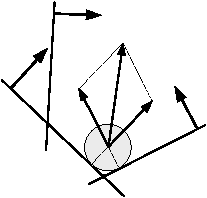
\includegraphics[scale=1]{part_1/chapter_5/figures/Figure1}};
		\node (c) at (0.3,1.1) {$c$};
		\node (a1) at (-1.2,1.0) {$a_1$};					
		\node (a2) at (1.65,0.1) {$a_2$};					
		\node (a3) at (-0.2,1.65) {$a_3$};
		\node (p1a1) at (0.7,0.2) {\small $p_1a_1$};					
		\node (p2a2) at (-0.4,0.4) {\small $p_2a_2$};				
		\node (x) at (0,-1.55) {\small $\overline{x}$};						
	\end{tikzpicture}			
	\caption{A geometric representation of duality for linear programming problems} \label{p1c5:fig:duality_geometry}	
\end{figure}

We can then think of the dual variables $p$ as the multipliers applied to the normal vectors associated with the hyperplanes (i.e., the walls) that are in contact with the particle to achieve this equilibrium. Hence, these multipliers $p$ will be such that
%
\begin{equation*}
c = \sum_{i \in I}p_ia_i, \text{ for some } p_i \geq 0, i \in I,	
\end{equation*}
%
which is precisely the dual feasibility condition (i.e., constraint) associated with the dual of $P$, given by
%
\begin{equation*}
	D : \maxi \braces{p^\top b : p^\top A = c, p \geq 0}.	
\end{equation*}
%
And, dual feasibility, as we seen before, implies the optimality of $\overline{x}$. 


\subsection{Complementary slackness}

One point that must be noticed is that, for the constraints that are not active at the optimal point $\overline{x}$ (i.e., the walls that are not exerting resistance to the particle at the equilibrium point), the multipliers $p$ must be set to zero. That is, we have that
%
\begin{equation*}
	p^\top b  = \sum_{i \in I} p_ib_i = \sum_{i \in I} p_i(a_i^\top\overline{x}) = c^\top \overline{x},	
\end{equation*}
%
which again implies the optimality of $p$ (cf. Corollary \ref{p1c5:cor:weak_duality} (3)). This geometrical insight leads to another key result for linear programming duality, which is the notion of \emph{complementary slackness}.

\begin{theorem}[Complementary slackness]
	Let $x$ be a feasible solution for 
	%
	\begin{equation*}
		(P) : \mini\braces{c^\top x : Ax = b, x \geq 0}	
	\end{equation*}
	%
	and $p$ be a feasible solution for 
	%
	\begin{equation*}
		(D) : \maxi\braces{p^\top b : p^\top A \leq c^\top}. 	
	\end{equation*}
	%
	The vectors $x$ and $p$ are optimal solutions to $P$ and $D$, respectively, if and only if
	$p_i(a_i^\top x - b_i) = 0, \forall i \in I$, and $(c_j - p^\top A_j)x_j = 0, \, \forall j \in J$. 
\end{theorem}

\begin{proof} 
	From the proof of Theorem \ref{p1c5:thm:weak_duality} and with Theorem \ref{p1c5:thm:strong_duality} holding, we have that 
%
	\begin{equation*}
		p_i(a_i^\top x - b_i) = 0, \forall i \in I, \text{ and } 	
	(c_j - p^\top A_j)x_j = 0, \, \forall j \in J.
	\end{equation*}
%
	In turn, if these hold, then $x$ and $p$ are optimal (cf. Corollary \ref{p1c5:cor:weak_duality} (3)). 
\end{proof}

For nondegenerate basic feasible solutions (BFS) (i.e., $x_j > 0$, $\forall j \in I_B$, where $I_B$ is the set of basic variable indices), complementary slackness determine a \emph{unique} dual solution. That is
%
\begin{equation*}
	(c_j - p^\top A_j)x_j = 0, \text{ which yields } c_j = p^\top A_j, \, \forall j \in I_B,
\end{equation*}
%
which has a unique solution $p^\top = c_B^\top B^{-1}$, as the columns $A_j$ of be are assumed to be linearly indepedent. In the presence of degeneracy, this is not the case anymore, typically implying that a degenerate optimal BFS will multiple feasible dual variable.


\subsection{Dual feasibility and optimality}

Combining what we have seen so far, the conditions for a \emph{primal-dual pair} $(x,p)$ to be optimal to their respective primal ($P$) and dual ($D$) problems are given by 
%
\begin{align}
	& a_i^\top x \geq b_i, \, \forall i \in I & & \text{(primal feasibility)}\label{p1c5:eq:primal_feas} \\
	& p_i = 0, \, \forall i \notin I^0   & & \text{(complementary conditions)} \label{p1c5:eq:cc}\\
	& \sum_{i \in I} p_i^\top a_i = c & & \text{(dual feasibility I)} \label{p1c5:eq:dual_feasI} \\
	& p_i \geq 0, & & \text{(dual feasibility II)} \label{p1c5:eq:dual_feasII}
\end{align}
%
where $I^0 = \braces{i \in I, a_i^\top x = b _i}$ are the active constraints. From \eqref{p1c5:eq:primal_feas}--\eqref{p1c5:eq:dual_feasII}, we see that the optimality of the primal-dual pair has two main requirements. The first is that $x$ must be (primal) feasible. The second, expressed as 
%
\begin{equation*}
	\sum_{i \in I^0} p_ia_i = c, \ p_i \geq 0,
\end{equation*}
%
is equivalent to requiring $c$ to be expressed as a nonnegative linear combination (also known as a conic combination) of the active constraints. This has a nice geometrical interpretation: dual feasibility can be seen as having the vector $c$ inside the ``cone'' formed by the normal vectors of the active constraints, which in turn is a necessary condition for the existence of an equilibrium, as described in Figure \ref{p1c5:fig:duality_geometry}. Figure \ref{p1c5:fig:dual_feasibility} illustrates this fact.

\begin{figure}
	\begin{tikzpicture}
%			\draw[help lines] (-4,-2) grid (4,2);
		\node (pic) at (0,0) {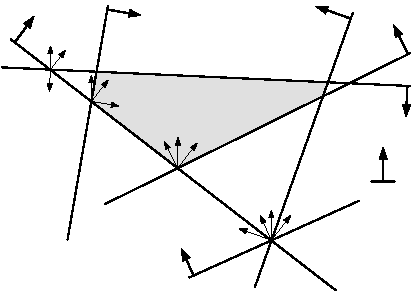
\includegraphics{part_1/chapter_5/figures/Figure2}};
		\node (A) at (-2.9,1.1) {$A$};
		\node (B) at (-2.2, 0.65) {$B$};
		\node (C) at (-0.5, -0.65) {$C$};
		\node (D) at (1.6, -1.6) {$D$};
		\node (c0) at (3.15, 0) {\footnotesize $c$};
		\node (c1) at (-2.7, 1.8) {\footnotesize $c$};
		\node (c2) at (-2.1, 1.15) {\footnotesize $c$};
		\node (c3) at (-0.5, 0.3) {\footnotesize $c$};
		\node (c4) at (1.1, -0.95) {\footnotesize $c$};
		\node (a11) at (-2.7, 2.2) {\footnotesize $a_1$};
		\node (a12) at (-2.2, 1.7) {\footnotesize $a_1$};
		\node (a13) at (-1.45, 1.1) {\footnotesize $a_1$};
		\node (a14) at (0, 0.1) {\footnotesize $a_1$};
		\node (a15) at (1.5, -1.05) {\footnotesize $a_1$};
		\node (a21) at (-0.9, 2.2) {\footnotesize $a_2$};
		\node (a22) at (-1.3, 0.7) {\footnotesize $a_2$};
		\node (a31) at (3.4, 2.2) {\footnotesize $a_3$};
		\node (a32) at (-0.9, 0.2) {\footnotesize $a_3$};
		\node (a41) at (3.4, 0.4) {\footnotesize $a_4$};
		\node (a42) at (-2.6, 0.8) {\footnotesize $a_4$};
		\node (a51) at (1.7, 2.3) {\footnotesize $a_5$};
		\node (a52) at (0.4, -1.4) {\footnotesize $a_5$};
		\node (a61) at (-0.5, -1.55) {\footnotesize $a_6$};
		\node (a62) at (0.8, -1.05) {\footnotesize $a_6$};
	\end{tikzpicture}
	\caption{$A$ is both primal and dual infeasible; $B$ is primal feasible and dual infeasible; $C$ is primal and dual feasible; $D$ is degenerate.} \label{p1c5:fig:dual_feasibility}
\end{figure}

Notice how in Figure \ref{p1c5:fig:dual_feasibility} neither points A or B are dual feasible, while C represents a dual feasible point, being thus the optimal for the problem depicted. One interesting point to notice is D. Although not feasible, it allows us to see an important effect that degeneracy may cause. Assume for a moment that D is feasible. Then, dual feasibility becomes dependent on the basis representing the vertex. That is,  while the bases $I_B = \braces{1,5}$ and $I_B = \braces{1,6}$ are dual feasible, the basis $I_B = \braces{5,6}$ is not. As we will see, just as it is the case with the simplex method, the dual simplex method, which we will discuss in the next section, might be subject to stalling and cycling from the presence of primal degeneracy, which in turn may also leads to multiple dual feasible (primal optimal) solutions.
 

\section{Practical uses of duality}

We now consider practical uses for the properties we have discussed in the previous section. The most direct application of duality in linear programming problems is the interpretation of dual variable values as marginal values associated with constraints, with important economical implications. 

Another important employment of duality consists of the development of an alternative variant of the simplex method, the \emph{dual simplex method}, which is particularly useful in several contexts.



\subsection{Optimal dual variables as marginal costs}

The optimal dual variable values associated with an optimal BFS have an important practical interpretation. To see that, let $\overline{x}$ be a nondegenerate optimal BFS with corresponding basis $B$. Thus, $\overline{x}_B = B^{-1}b > 0$.

Now, assume that we cause a marginal perturbation on the vector $b$, represented by a vector $d$. That is, assume that we have $B^{-1}(b + d) > 0$, noticing that nondegenerate feasibility holds.

Recall that the optimality condition $\overline{c} = c^\top - c_B ^\top B^{-1}A \geq 0$ is not influenced by such a marginal perturbation. That is, for a small change $d$, the optimal basis (i.e., the selection of which the are basic variables) is not disturbed. On the other hand, the optimal value of the basic variables is, and consequently, so is the optimal value, which becomes
%
\begin{equation*}
	c_B^\top B^{-1}(b + d) = p^\top(b + d). 
\end{equation*}
%
Notice that $p^\top = c_B^\top B^{-1}$ is optimal for the (respective) dual problem. Thus, a change $d$ causes a change of $p^\top d$ in the optimal value, meaning that the components $p_i$ represent a marginal value/cost associated with the independent term $b_i$, for $i \in I$. 

This has important implications in practice, as it allows for pricing the the values of the resources associated with constraints. For example, if the dual value (or price) $p_i$ is associated with a resource whose requirement is given by $b_i$, this means that any opportunity of removing any units of $b_i$ for less than $p_i$ should be seized, since it costs $p_i$ to satisfy any additional unit in the requirement $b_i$. A similar interpretation can be made in the context of less-or-equal-than constraints, in which $p_i$ would indicate benefits (or loses, if $p_i > 0$) in increasing the availability of $b_i$. 

% TODO: A simple numerical example coming back to the paint example would be helpful here

\subsection{The dual simplex method}

In general, solution methods in mathematical programming can be either \emph{primal methods}, in which primal feasibility of an initial solution is maintained while seeking for dual feasibility (i.e., primal optimality); or \emph{dual methods}, where dual feasibility is maintained while seeking for primal feasibility (i.e., dual optimality).

As we have seen in Chapter \ref{chapter_4}, the original (or primal) simplex method iterated from an initial basic feasible solution (BFS) until the optimality condition 
%
\begin{equation*}
	\overline{c} = c^\top - c_BB^{-1}A \geq 0
\end{equation*}
%
was observed. Notice that this condition is precisely the dual feasibility condition $p^\top A \leq c$. 

Being a dual method, the dual version of the simplex method, or the \emph{dual simplex method}, consider conditions in a reverse order. That is, it starts from an initial dual feasible solution and iterates in a manner that the primal feasibility condition $B^{-1}b \geq 0$ is \emph{sought} for, while $\overline{c} \geq 0$, or equivalently, $p^\top A \leq c$, is maintained.

To achieve that, one must revise the pivoting of the primal simplex method such that the variable to leave the basis is some $i \in I_B$, with $x_{B(i)} < 0$, while the variable chosen to enter the basis is some $j \in I_N$, such that $\overline{c} \geq 0$ is maintained.

 Consider the $l^\text{th}$ simplex tableau row for which $x_{B(i)} < 0$ of the form $[v_1,\dots, v_n, x_{B(i)}]$; i.e., $v_j$ is the $l^\text{th}$ component of $B^{-1}A_j$.
	 
 For each $j \in I_N$ for which $v_j < 0$, we pick
 %
 \begin{equation*}
 	j' = {\arg\min}_{j \in I_N : v_j < 0} \frac{\overline{c}_j}{|v_j|}.	
 \end{equation*}
 %
 Pivoting is performed by employing elemental row operations to replace $A_{B(i)}$ with $A_j$ in the basis. This implies that $\overline{c}_j \geq 0$ is maintained, since
 %
 \begin{equation*}
	\frac{\overline{c}_j}{|v_j|} \geq \frac{\overline{c}_{j'}}{|v_{j'}|} \Rightarrow \overline{c}_j -|v_j|\frac{\overline{c}_{j'}}{|v_{j'}|} \geq 0 \Rightarrow \overline{c}_j + v_j\frac{\overline{c}_{j'}}{|v_{j'}|} \geq 0, \, \forall j \in J.
 \end{equation*}
%
Notice that it also justifies why we must only consider for entering the basis those variables for which $v_j < 0$. Analogously to the case in the primal simplex method, if we observe that $v_j \ge 0$ for all $j \in J$ , then no limiting condition is imposed in terms the increase in the nonbasic variable (i.e., an unbounded dual, which, according to Corollary \ref{p1c5:cor:weak_duality} (2), implies the original problem is infeasible).

Assuming that the dual is not unbounded, the termination of the dual simplex method is observed when $B^{-1}b \geq 0$ is achieved, and primal-dual optimal solutions have been found, with $x = (x_B,x_N) = (B^{-1}b, 0)$ (i.e., the primal solution) and $p = (p_B, p_N) = (0, c_B^\top B^{-1})$ (dual). Algorithm \ref{p1c5:alg:dual_simplex} presents a pseudocode for the dual simplex method.

\begin{algorithm}[h]
	\caption{Dual simplex method} \label{p1c5:alg:dual_simplex}
	\begin{algorithmic}[1] %line numbering frequency. 
		\State {\bf initialise.} Initial basis $B$ and associated basic solution $x$.
		\While {$x_B = B^{-1}b < 0$ for some component $i \in I_B$} \label{alg:opt_condition} 
			\State Choose some $l$ for which $x_{B(l)} < 0$. Calculate $u = B^{-1}A_j$. 
			\If {$u \geq 0$} \label{alg:unb_condition}
				\State {\bf return} $z = +\infty$.		
			\Else
				\State Form new basis $B = B \setminus \braces{l} \cup \braces{j'}$ where $j' = \arg\min_{j \in I_N : u_j < 0} \frac{\overline{c}_j}{|u_j|}$ 
				\State Calculate $x_B = B^{-1}b$.
			\EndIf
		\EndWhile
		\State {\bf return} optimal basis $B$ and optimal solution $x$.
	\end{algorithmic}
\end{algorithm}

To clarify some of the previous points, let us consider a numerical example. Consider the problem 
%
\begin{align*}
	\mini &x_1 + x_2 \\
	\st &x_1 + 2x_2 \geq 2 \\
	&x_1 \geq  1 \\
	&x_1,x_2,x_3,x_4 \geq 0.	
\end{align*}	
%
The first thing we must do is to convert the greater-or-equal-than inequalities into less-or-equal-than inequalities and add the respective slack variables. This allows us to avoid the inclusion of artificial variables, which are not required anymore since we can allow for primal infeasibility. This leads to the equivalent standard form problem
%
\begin{align*}
	\mini &x_1 + x_2 \\
	\st &-x_1 - 2x_2 + x_3 = -2 \\
	&-x_1 + x_4 = -1 \\
	&x_1,x_2,x_3,x_4 \geq 0.	
\end{align*}

Below is the sequence of tableaus after applying the dual simplex method to solve the problem. The terms in bold font represent the pivot element (i.e., the intersection between the pivot row and pivot column). 

% TODO: some pretty editing to make the column width match among tables.

\begin{center}
	\begin{tabular}{c|cccc|c}
		 & $x_1$ & $x_2$ & $x_3$ & $x_4$ & RHS \\ \hline 
		$z$  &  1 & 1 & 0 & 0 & 0  \\ \hline
	   $x_3$ & -1 &\textbf{-2} & 1 & 0 & -2 \\
	   $x_4$ & -1 & 0 & 0 & 1 & -1 \\\hline \hline
	\end{tabular}
	
	\begin{tabular}{c|cccc|c}
		 & $x_1$ & $x_2$ & $x_3$ & $x_4$ & RHS \\ \hline 
		$z$  & 1/2 & 0 & 1/2 & 0 & -1  \\ \hline
	   $x_2$ & 1/2 & 1 & -1/2 & 0 & 1 \\
	   $x_4$ & \textbf{-1} & 0 & 0 & 1 & -1 \\ \hline \hline 
	\end{tabular}
	
	\begin{tabular}{c|cccc|c}
		 & $x_1$ & $x_2$ & $x_3$ & $x_4$ & RHS \\ \hline 
		$z$  & 0 & 0 & 1/2 & 1/2 & -3/2  \\ \hline
	   $x_2$ & 0 & 1 & -1/2 & 1/2 & 1/2 \\
	   $x_1$ & 1 & 0 & 0 & -1 & 1 \\ \hline 
	\end{tabular}
\end{center}

Figure \ref{p1c5:fig:ex1} illustrates the progress of the algorithm both in the primal (Figure \ref{p1c5:fig:ex1_P}) and in the dual (Figure \ref{p1c5:fig:ex1_D}) variable space. Notice how in the primal space the solution remains primal infeasible until a primal feasible solution is reached, that being the optimal for the problem. Also, notice that the coordinates of the dual variables can be extracted from the zeroth row of the simplex tableau.

\begin{figure}[h]
	\centering
	\begin{subfigure}{0.45\textwidth}
		\centering
		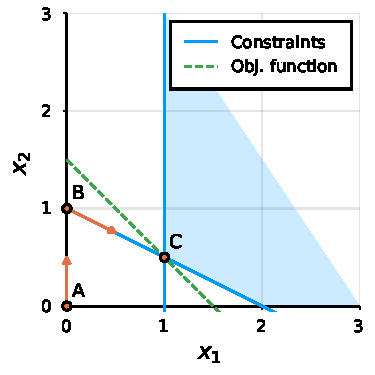
\includegraphics{part_1/chapter_5/figures/primal_plot}
		\caption{The primal-variable space}\label{p1c5:fig:ex1_P}
	\end{subfigure}
	\begin{subfigure}{0.45\textwidth}
		\centering
		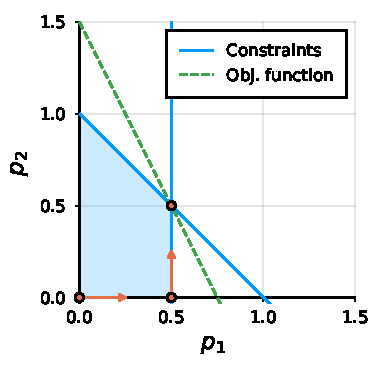
\includegraphics{part_1/chapter_5/figures/dual_plot}
		\caption{The dual-variable space}\label{p1c5:fig:ex1_D}
	\end{subfigure}
	\caption{The progress of the dual simplex method in the primal and dual space.}	\label{p1c5:fig:ex1}
\end{figure}

Some interesting features related to the progress of the dual simplex algorithm are worth highlighting. First, notice that the objective function is monotonically increasing in this case, since $x_{B(l)}\frac{\overline{c}_{j'}}{|v_{j'}|}$ is added to $-c_BB^{-1}b$ and $x_{B(l)} < 0$, meaning that the dual cost increases (recall the convention of having a minus sign so that the zeroth row correctly represent the objective function value, given by the negative of the value displayed in the rightmost column). This illustrates the gradual loss of optimality in the search for (primal) feasibility. For a nondegerate problem, this can also be used as an argument for eventual convergence, since the dual objective value can only increase and is bounded by the primal optimal value. However, in the presence of dual degeneracy, that is, $\overline{c}_{j} = 0$ for some $j \in I_N$ in the optimal solution, the algorithm can suffer from cycling. As we seen before, that is an indication that the primal problem has multiple optima. 

The dual simplex method is often the best choice of algorithm, because it typically precludes the need of a Phase I type of method as it is often trivial to find initial dual feasible solutions (the origin, for example, is typically dual feasible in minimisation problems with nonnegative coefficients; similar trivial cases are also well known).

Moreover, dual simplex is the algorithm of choice for resolving a linear programming problem when after finding an optimal solution, you modify the feasible region. Turns out that this procedure is in the core of the methods used to solve integer programming problems, as well as in the Benders decomposition, both topics we will explore later on. The dual simplex method is also more successful than its primal counterpart in combinatorial optimisation problems, which are typically plagued with degeneracy. As we have seen, primal degeneracy simply means multiple dual optima, which are far less problematic under an algorithmic standpoint.

Most professional implementations of the simplex method use by default the dual simplex version. This has several computational reasons, in particular related to more effective Phase I and pricing methods for the dual counterpart.

 
\section{Exercises}

\subsection*{Exercise 5.1: Duality in the transportation problem}
Recall Exercise 1.4 in which we solved a capacitated transportation problem, answer the following questions based on the dual prices interpretation. The tables with the arc capacities and supply/demand settings are once more presented in Tables \ref{table:c5_supdem} and \ref{table:c5_arcs}.

\begin{table}[h!]
	\begin{subtable}[h]{0.4\textwidth}
		\begin{center}
		\begin{tabular}{c|cc}
			\textbf{node} & \textbf{p1} & \textbf{p2} \\
			\hline
			\textbf{s1 / d1} & 80 / 60 & 400 / 300 \\
			\textbf{s2 / d2} & 200 / 100 & 1500 / 1000 \\
			\textbf{s3 / d3} & 200 / 200 & 300 / 500 \\
		\end{tabular}
		\end{center}
		\caption{Supplies availability and demand per oil type [in L]}
		\label{table:c5_supdem}
	\end{subtable}
	\hfill
	\begin{subtable}[h]{0.55\textwidth}
		\begin{center}
			\begin{tabular}{c|ccc}
				 & \textbf{d1} & \textbf{d2} & \textbf{d3}\\
				 & \textbf{p1/p2 (cap)} & \textbf{p1/p2 (cap)} & \textbf{p1/p2 (cap)}\\
				\hline
				\textbf{s1} & 5/- ($\infty$) & 5/18 (300) & -/- (0)\\
				\textbf{s2} & 8/15 (300) & 9/12 (700) & 7/14 (600)\\
				\textbf{s3} & -/- (0) & 10/20 ($\infty$) & 8/- ($\infty$)\\
			\end{tabular}
		\end{center}
		\caption{Arcs costs per oil type [in \euro \ per L] and arcs` capacities [in L]}
		\label{table:c5_arcs}
	\end{subtable}
	\caption{Supply chain data}
	\label{table:c5_sc}
\end{table}
%
\begin{itemize}
	\item [(a)] What would be the price the company would be willing to pay for raising in one unit any of the supplies availability?

	\item [(b)] What would be the price the company would be willing to pay for raising in one unit any of the arcs capacity?	
\end{itemize}


\subsection*{Exercise 5.2: Dual simplex}
\begin{itemize}
\item[(a)] Solve the problem below by using the dual Simplex method. Report both the primal and dual optimal solutions $x$ and $p$ associated with the optimal basis.
\item[(b)] Write the dual and use duality to verify that $x$ and $p$ are optimal.
\end{itemize}
%
\begin{align*}
	\mini & 2x_1 + x_3  \\
	\st & -1/4 x_1 - 1/2 x_2 \leq -3/4 \\
	& 8x_1 + 12 x_2 \leq 20 \\
	& x_1 + 1/2 x_2 - x_3 \leq -1/2 \\
	& 9x_1 + 3 x_2 \geq -6 \\
	& x_1, x_2, x_3 \geq 0.
\end{align*}


\subsection*{Exercise 5.3: Unboundedness and duality}
\noindent Consider the LP:
\begin{align*}
	(P) : \mini & c^\top x \\
	\st & Ax = b \\
				& x \ge 0
\end{align*}
where $A \in \reals^{m \times n}$ and $b \in \reals^m$. Show that if $P$ has a finite optimal solution, then the new problem $\overline{P}$ obtained from $P$ by replacing the right hand side vector $b$ with another one $\bar{b} \in \reals^m$ cannot be unbounded no matter what value the components of $\bar{b}$ can take.


\subsection*{Exercise 5.4: Dual in matrix form}
\noindent Consider the LP:
\begin{align*}
	(P) : \mini &  {c^1}^\top x^1 + {c^2}^\top x^2 + {c^3}^\top x^3 & \\
	\text{s.t.} & \\ 
	 & {A}^1{x}^1 + {A}^2{x}^2 + {A}^3{x}^3 \leq b^1 \quad (y^1) \\
	 & {A}^4{x}^1 + {A}^5{x}^2 + {A}^6{x}^3 \leq b^2 \quad (y^2) \\	 
	 & {A}^7{x}^1 + {A}^8{x}^2 + {A}^9{x}^3 \leq b^3 \quad (y^3) \\
	 & x^1 \leq 0 \\
	 & x^2 \geq 0 \\
	 & x^3  \in \reals^{|x^3|}
\end{align*}

\noindent where $A^{1,...,9}$ are matrices, $b^{1,...,3}$, $c^{1,...,3}$ are column vectors, and $y^{1,...,3}$ are the dual variables associated to each constraint. 

\begin{itemize}
	\item[(a)] Write the dual problem in matrix form.
	
	\item[(b)] Compute the dual optimum for the case in which
	
	$
	A^1 = 
	\begin{bmatrix}
		1 & 2 \\
		3 & 4
	\end{bmatrix}  ; \ 
	A^2 = 
	\begin{bmatrix}
		5 & 1 \\
		0 & 0
	\end{bmatrix}  ; \ 
	A^3 = 
	\begin{bmatrix}
		6 \\
		0
	\end{bmatrix}  ; \ 
	A_4 = 
	\begin{bmatrix}
		1 & 1
	\end{bmatrix}  ; \ 
	A^5 = 
	\begin{bmatrix}
		0 & 1
	\end{bmatrix}  ; \ 
	A^6 = 
	\begin{bmatrix}
		1
	\end{bmatrix}  ; \\ 
	A^7 = 
	\begin{bmatrix}
		0 & 2
	\end{bmatrix}  ; \ 
	A^8 = 
	\begin{bmatrix}
		0 & 0
	\end{bmatrix}  ; \ 
	A^9 = 
	\begin{bmatrix}
		3
	\end{bmatrix}  ; \ 
	c^1 = 
	\begin{bmatrix}
		3 \\
		9
	\end{bmatrix}  ; \ 
	c^2 = 
	\begin{bmatrix}
		4 \\
		2
	\end{bmatrix}  ; \ 
	c^3 = 
	\begin{bmatrix}
		1
	\end{bmatrix}  ; \ 
	b^1 = 
	\begin{bmatrix}
		5 \\
		10
	\end{bmatrix}  ; \\ 
	b^2 = 
	\begin{bmatrix}
		3 
	\end{bmatrix}  ; \ 
	b^3 =
	\begin{bmatrix}
		6
	\end{bmatrix}
	$
	.
		
\end{itemize}


\subsection*{Exercise 5.5: Primal-dual conversion and complementary slackness}
Recall the paint factory problem introduced in Section \ref{section_121}.

\begin{itemize}
\item[(a)] Construct the dual of the problem below and solve both the original problem and its dual. 
\item[(b)] Use complementary slackness to verify that the primal and dual solutions are optimal.
\end{itemize}
%
\begin{align*}
	\maxi z = \ & 5x_1 + 4x_2 \\
	\st & 6x_1 + 4x_2 \leq 24 \\
	& x_1 + 2x_2 \leq 6 \\
	& x_2 - x_1 \leq 1 \\
	& x_2 \leq 2 \\
	& x_1, x_2 \geq 0.
\end{align*}





